% FSB Seminar — Sveučilište u Zagrebu, Fakultet strojarstva i brodogradnje
% Template v2.1 — latex_architect popunjava placeholdere iz project.yaml

\documentclass[12pt,a4paper]{article}

% --- Encoding, Font & Language (dual-engine) ---
% Kanonski engine je Tectonic (XeTeX): fontspec + TeX Gyre Termes ima PRAVI
% OpenType bold pa hrvatski ž/ć/š/đ rade i u \textbf{}. pdfLaTeX fallback koristi
% newtxtext (vidi gotcha miktex-t1-bold-diacritics). NE newtxmath uz amssymb (\Bbbk konflikt).
\usepackage{iftex}
\ifPDFTeX
  \usepackage[utf8]{inputenc}
  \usepackage[T1]{fontenc}
  \usepackage{newtxtext}
\else
  \usepackage{fontspec}
  \setmainfont{texgyretermes-regular.otf}[
    BoldFont       = texgyretermes-bold.otf,
    ItalicFont     = texgyretermes-italic.otf,
    BoldItalicFont = texgyretermes-bolditalic.otf
  ]
\fi
\usepackage[croatian]{babel}

% --- Layout ---
\usepackage[top=2.5cm,bottom=2.5cm,left=2.5cm,right=2.5cm]{geometry}
\usepackage{setspace}
\onehalfspacing

% --- Headers & Footers ---
\usepackage{fancyhdr}
\setlength{\headheight}{13.6pt}
\pagestyle{fancy}
\fancyhf{}
\fancyhead[L]{\small\itshape \authorname}
\fancyhead[R]{\small\itshape \seminartitleshort}
\fancyfoot[L]{\small\itshape Fakultet strojarstva i brodogradnje}
\fancyfoot[R]{\small\itshape\thepage}
\renewcommand{\headrulewidth}{0.4pt}
\renewcommand{\footrulewidth}{0.4pt}

% --- Section Formatting (14pt Bold Uppercase) ---
\usepackage{titlesec}
\titleformat{\section}
  {\normalfont\fontsize{14}{17}\bfseries\raggedright\MakeUppercase}
  {\thesection.}{0.5em}{}
\titleformat{\subsection}
  {\normalfont\fontsize{12}{15}\bfseries}
  {\thesubsection.}{0.5em}{}
\titleformat{\subsubsection}
  {\normalfont\fontsize{12}{15}\bfseries\itshape}
  {\thesubsubsection.}{0.5em}{}
\titleformat{\paragraph}[runin]
  {\normalfont\fontsize{12}{15}\itshape}
  {}{0em}{}[.]

% --- Figures & Tables ---
\usepackage{graphicx}
\usepackage{booktabs}
\usepackage{tabularx}
\usepackage{longtable}
\usepackage{array}
\usepackage{float}
\usepackage{caption}
\captionsetup[figure]{font={small,bf},labelsep=period,position=below}
\captionsetup[table]{font={small,bf},labelsep=period,position=above}

% --- Figure/Table numbering by section (Slika 2.1, Tablica 2.1) ---
\usepackage{chngcntr}
\counterwithin{figure}{section}
\counterwithin{table}{section}
\counterwithin{equation}{section}

% --- Depth ---
\setcounter{secnumdepth}{4}
\setcounter{tocdepth}{4}

% --- Croatian names (addto — babel croatian overrida renewcommand) ---
\addto\captionscroatian{%
  \renewcommand{\figurename}{Slika}%
  \renewcommand{\tablename}{Tablica}%
  \renewcommand{\contentsname}{\normalfont\fontsize{14}{17}\bfseries SADRŽAJ}%
  \renewcommand{\listfigurename}{\normalfont\fontsize{14}{17}\bfseries POPIS SLIKA}%
  \renewcommand{\listtablename}{\normalfont\fontsize{14}{17}\bfseries POPIS TABLICA}%
  \renewcommand{\refname}{\normalfont\fontsize{14}{17}\bfseries LITERATURA}%
}

% --- References ---
\usepackage{cite}

% --- Hyperlinks ---
\usepackage[hidelinks,unicode]{hyperref}

% --- Math ---
\usepackage{amsmath}
\usepackage{amssymb}

% --- Color (za upozorenja o nepopunjenim placeholderima) ---
\usepackage{xcolor}

% --- Ispis MATLAB koda ---
\usepackage{listings}
\lstdefinestyle{matlabstil}{
  language=Matlab,
  basicstyle=\ttfamily\scriptsize,
  keywordstyle=\color[rgb]{0,0,0.6}\bfseries,
  commentstyle=\color[rgb]{0,0.45,0}\itshape,
  stringstyle=\color[rgb]{0.65,0.15,0.15},
  numbers=left, numberstyle=\tiny\color{gray}, numbersep=7pt,
  frame=single, rulecolor=\color{gray},
  breaklines=true, breakatwhitespace=false,
  showstringspaces=false, tabsize=4,
  columns=fullflexible, keepspaces=true,
  captionpos=b,
  extendedchars=true, inputencoding=utf8, literate=%
    {č}{{\v{c}}}1 {ć}{{\'c}}1 {ž}{{\v{z}}}1 {š}{{\v{s}}}1 {đ}{{\dj}}1
    {Č}{{\v{C}}}1 {Ć}{{\'C}}1 {Ž}{{\v{Z}}}1 {Š}{{\v{S}}}1 {Đ}{{\DJ}}1
}
\lstset{style=matlabstil}
\renewcommand{\lstlistingname}{Kod}

% --- Paragraph spacing ---
\setlength{\parindent}{1.25cm}
\setlength{\parskip}{0pt}

% --- Spriječavanje razdvajanja riječi (Justify bez hifenacije) ---
\hyphenpenalty=10000
\exhyphenpenalty=10000
\tolerance=10000
\hbadness=10000
\emergencystretch=\maxdimen

% ============================================================
% DOCUMENT METADATA — latex_architect popunjava iz project.yaml
% ============================================================
\newcommand{\univname}{SVEUČILIŠTE U ZAGREBU}
\newcommand{\facultyname}{FAKULTET STROJARSTVA I BRODOGRADNJE}
\newcommand{\coursename}{OPTIMIZACIJSKE METODE U RAZVOJU I UPRAVLJANJU SUSTAVA}
\newcommand{\seminartitle}{Kvadratično programiranje, robusna optimizacija i robusna stabilizacija dinamičkih sustava}
\newcommand{\seminartitleshort}{QP, robusna optimizacija i stabilizacija}
\newcommand{\professorname}{Prof. dr. sc. Andrej Jokić}
\newcommand{\authorname}{Ivan Noršić}
% Predložak nema polje za matični broj; definirano ovdje ručno. Ako se
% docs/main.tex ikad ponovno generira s render_template.py --force, vratiti.
\newcommand{\studentid}{0035239736}
\newcommand{\locationdate}{Zagreb, 2026.}

% ============================================================
\begin{document}

% ---- TITLE PAGE ----
\begin{titlepage}
  \centering
  {\fontsize{14}{17}\selectfont \univname \par}
  {\fontsize{14}{17}\selectfont \facultyname \par}
  \vfill
  {\fontsize{28}{34}\bfseries \coursename \par}
  \vspace{0.8cm}
  {\fontsize{14}{18}\bfseries \seminartitle \par}
  \vfill
  % Tabular: lijevo "Profesor:" / bold ime — desno "Student:" / bold ime
  % \textmd i \textbf (ne \bfseries/\normalfont — ne rade pouzdano u p{} ćelijama)
  \begin{tabular}{p{0.45\textwidth}>{\raggedleft\arraybackslash}p{0.45\textwidth}}
    \textmd{Profesor:} & \textmd{Student:} \\[0.3cm]
    \textbf{\professorname} & \textbf{\authorname} \\[0.25cm]
                            & \textmd{Mat.~broj: \studentid}
  \end{tabular}
  \vspace{1.5cm}
  \par
  {\normalfont \locationdate \par}
\end{titlepage}

% ---- FRONTMATTER (rimske stranice velikim slovima: I, II, III) ----
\pagenumbering{Roman}
\setcounter{page}{1}

\tableofcontents
\clearpage



% ---- BODY (arapske stranice) ----
\pagenumbering{arabic}
\setcounter{page}{1}

% 00 — Uvod.

\section{Uvod}
\label{sec:uvod}

Ovaj seminarski rad obrađuje četiri zadatka iz kolegija \emph{Optimizacijske
metode u razvoju i upravljanju sustava} \cite{jokic_zadatak}. Iako se zadaci na
prvi pogled bave različitim temama --- od kvadratnog programa s dva ograničenja
do stabilizacije hibridnog dinamičkog sustava --- povezuje ih zajednička nit:
svaki se svodi na \emph{konveksan} optimizacijski problem, za koji lokalni
optimum ujedno je i globalni, a uvjeti optimalnosti su i nužni i dovoljni
\cite[str.~61]{jokic_konveksnost}.

Poglavlje~\ref{sec:zad1} obrađuje kvadratni program s linearnim ograničenjima.
Analizira se konveksnost, postavljaju se i analitički rješavaju
Karush--Kuhn--Tuckerovi uvjeti \cite[str.~59]{jokic_kkt}, rezultat se provjerava
funkcijom \texttt{quadprog} i modeliranjem u YALMIP-u, te se postavlja i rješava
Lagrangeov dualni problem. Na kraju se pokazuje kako Lagrangeovi množitelji
mjere osjetljivost optimalne vrijednosti na perturbacije ograničenja.

Poglavlje~\ref{sec:zad2} isti problem promatra uz nesigurne koeficijente
ograničenja. Pokazuje se da se zahtjev dopustivosti za sve realizacije svodi na
konačan skup ograničenja najgoreg slučaja i da robusna protuformulacija ostaje
konveksna, pa se rješava istim alatom. Kvantificira se i cijena robusnosti.

Poglavlje~\ref{sec:zad3} bavi se oblikovanjem profila ceste na neravnom terenu.
Naglasak je na \emph{formulaciji}: pokazuje se da izbor mjere troška određuje
klasu problema, te da diskretizacija derivacija podijeljenim razlikama zadržava
linearnost i vodi na linearni program.

Poglavlje~\ref{sec:zad4} prelazi na dinamičke sustave. Analizira se prekidački
sustav s dva stabilna moda koji je unatoč tome nestabilan, i sintetizira se
statički regulator koji ga stabilizira. Sinteza se oslanja na zajedničku
kvadratnu Ljapunovljevu funkciju \cite[str.~4]{jokic_ljapunov}, čime se problem
upravljanja svodi na sustav linearnih matričnih nejednakosti.

Svi numerički rezultati dobiveni su u MATLAB-u, po jednom skriptom za svaki
zadatak. Skripte su u cijelosti navedene u prilogu (poglavlje~\ref{sec:kod}), a
nalaze se i u direktoriju \texttt{src/} repozitorija; reproduciraju sve brojeve
i slike iz ovog rada.


% 01 — Zadatak 1: QP, konveksnost, KKT, dualnost.

\section{Zadatak 1 --- kvadratično programiranje, KKT uvjeti i dualnost}
\label{sec:zad1}

\subsection{Formulacija problema}
\label{sec:zad1:formulacija}

Zadan je optimizacijski problem \cite[str.~1]{jokic_zadatak}
\begin{align}
  \min_{x}\quad & x_1^2 + 2x_2^2 - 0{,}3\,x_1x_2 + 2x_1 - 3x_2 \label{eq:z1cilj}\\
  \text{uz}\quad & a_{11}x_1 + a_{12}x_2 \le -10, \label{eq:z1g1}\\
                 & a_{21}x_1 + a_{22}x_2 \le 3, \label{eq:z1g2}
\end{align}
uz $a_{11}=-1$, $a_{12}=-1$, $a_{21}=1$, $a_{22}=-1$. Uvrštavanjem numeričkih
vrijednosti ograničenja postaju $x_1 + x_2 \ge 10$ i $x_1 - x_2 \le 3$.

Problem zapisujemo u standardnoj formi kvadratnog programa
$f(x) = \tfrac{1}{2}x^{\mathsf T}Hx + c^{\mathsf T}x$ uz $Ax \le b$
\cite[str.~34]{jokic_lpqp}, gdje je
\begin{equation}
  H = \begin{bmatrix} 2 & -0{,}3 \\ -0{,}3 & 4 \end{bmatrix}, \quad
  c = \begin{bmatrix} 2 \\ -3 \end{bmatrix}, \quad
  A = \begin{bmatrix} -1 & -1 \\ 1 & -1 \end{bmatrix}, \quad
  b = \begin{bmatrix} -10 \\ 3 \end{bmatrix}.
  \label{eq:z1std}
\end{equation}
Faktor $\tfrac12$ je nužan: dijagonalni članovi $H$ su dvostruki koeficijenti
kvadratnih članova, a izvandijagonalni je polovica koeficijenta mješovitog člana.

\subsection{Analiza konveksnosti}
\label{sec:zad1:konveksnost}

Funkcija cilja je konveksna ako i samo ako je njezina Hesseova matrica pozitivno
semidefinitna \cite[str.~61]{jokic_konveksnost}. Ovdje je $\nabla^2 f(x) = H$,
konstantna, sa svojstvenim vrijednostima
\begin{equation}
  \lambda(H) = \{1{,}955969,\; 4{,}044031\},
\end{equation}
dakle obje strogo pozitivne. Do istog zaključka vodi i Sylvesterov kriterij:
vodeći glavni minori su $2 > 0$ i $\det H = 8 - 0{,}09 = 7{,}91 > 0$.

Matrica $H$ je stoga pozitivno definitna, pa je $f$ \emph{strogo} konveksna.
Ograničenja \eqref{eq:z1g1}--\eqref{eq:z1g2} su linearna, pa je dozvoljeni skup
presjek dvaju poluravnina --- konveksan poliedar. Riječ je dakle o konveksnom
optimizacijskom problemu, i to strogo konveksnom QP-u. Posljedice su bitne za
sve što slijedi: rješenje je jedinstveno ako postoji, svaki lokalni minimum je
ujedno i globalni, a KKT uvjeti su ne samo nužni nego i \emph{dovoljni}.

\subsection{KKT uvjeti optimalnosti i njihovo rješenje}
\label{sec:zad1:kkt}

Uz Lagrangeovu funkciju $L(x,\lambda) = f(x) + \lambda^{\mathsf T}(Ax-b)$,
KKT uvjeti \cite[str.~59]{jokic_kkt} glase
\begin{align}
  Hx + c + A^{\mathsf T}\lambda &= 0 && \text{(stacionarnost)}, \label{eq:kkt1}\\
  Ax - b &\le 0 && \text{(primarna dopustivost)}, \\
  \lambda &\ge 0 && \text{(dualna dopustivost)}, \\
  \lambda_i\,(A_ix - b_i) &= 0,\quad i=1,2 && \text{(komplementarnost)}. \label{eq:kkt4}
\end{align}

Uvjet komplementarnosti \eqref{eq:kkt4} znači da je svako ograničenje ili
aktivno ($A_ix = b_i$, uz $\lambda_i \ge 0$) ili neaktivno ($A_ix < b_i$, uz
$\lambda_i = 0$). Sustavan postupak je stoga proći kroz sve $2^m$ kombinacija
aktivnih skupova i potražiti onu koja zadovoljava \emph{sve} KKT uvjete. Uz
$m = 2$ ograničenja to su četiri slučaja. Za pretpostavljeni aktivni skup $S$
rješava se linearan sustav
\begin{equation}
  \begin{bmatrix} H & A_S^{\mathsf T} \\ A_S & 0 \end{bmatrix}
  \begin{bmatrix} x \\ \lambda_S \end{bmatrix}
  = \begin{bmatrix} -c \\ b_S \end{bmatrix},
  \label{eq:kktsys}
\end{equation}
a zatim se provjeravaju primarna dopustivost $Ax \le b$ i dualna dopustivost
$\lambda \ge 0$. Rezultati su u tablici~\ref{tab:z1cases}.

\begin{table}[htbp]
  \centering
  \caption{Nabrajanje aktivnih skupova. Točno jedan slučaj zadovoljava sve KKT uvjete.}
  \label{tab:z1cases}
  \begin{tabular}{lccl}
    \hline
    Aktivni skup & $x$ & $\lambda$ & Status \\
    \hline
    $\{\}$          & $(-0{,}8976,\; 0{,}6827)$ & $(0,\; 0)$ & odbačen: nedopustiv \\
    $\{g_1\}$       & $(5{,}7576,\; 4{,}2424)$  & $(12{,}2424,\; 0)$ & \textbf{zadovoljava sve} \\
    $\{g_2\}$       & $(2{,}2407,\; -0{,}7593)$ & $(0,\; -6{,}7093)$ & odbačen: nedopustiv \\
    $\{g_1, g_2\}$  & $(6{,}5000,\; 3{,}5000)$  & $(11{,}5000,\; -2{,}4500)$ & odbačen: $\lambda_2 < 0$ \\
    \hline
  \end{tabular}
\end{table}

Slučaj bez aktivnih ograničenja daje bezuvjetni minimum $-H^{-1}c$, koji je
nedopustiv jer je $x_1 + x_2 = -0{,}215 < 10$. Slučaj $\{g_2\}$ je također
nedopustiv, a slučaj s oba aktivna ograničenja daje negativan množitelj
$\lambda_2 = -2{,}45$, čime pada na dualnoj dopustivosti. Preostaje jedini
kandidat
\begin{equation}
  x^\star = \begin{bmatrix} 190/33 \\ 140/33 \end{bmatrix}
          = \begin{bmatrix} 5{,}757576 \\ 4{,}242424 \end{bmatrix}, \qquad
  \lambda_1^\star = \frac{404}{33} = 12{,}242424, \qquad \lambda_2^\star = 0 .
  \label{eq:z1sol}
\end{equation}

Za njega je $\lambda_1^\star > 0$, drugo ograničenje je neaktivno jer je
$x_1^\star - x_2^\star - 3 = -1{,}484848 < 0$, što je konzistentno s
$\lambda_2^\star = 0$ u \eqref{eq:kkt4}, a rezidual stacionarnosti iznosi
$\lVert Hx^\star + c + \lambda_1^\star A_1^{\mathsf T}\rVert \approx 1{,}8\cdot10^{-15}$.
Optimalna vrijednost je
\begin{equation}
  p^\star = f(x^\star) = \frac{2000}{33} = 60{,}606061 .
\end{equation}
Budući da je problem konveksan, KKT uvjeti su dovoljni, pa je $x^\star$ globalni
minimizator, a zbog stroge konveksnosti i jedini.

\subsection{Grafički prikaz dozvoljenog skupa i gradijenata}
\label{sec:zad1:graficki}

Slika~\ref{fig:z1} prikazuje dozvoljeni skup, nivo krivulje funkcije cilja te
gradijente u točki $x^\star$. Gradijenti su
\begin{equation}
  \nabla f(x^\star) = Hx^\star + c = \begin{bmatrix} 12{,}242424 \\ 12{,}242424 \end{bmatrix}, \qquad
  \nabla g_1(x^\star) = \begin{bmatrix} -1 \\ -1 \end{bmatrix}, \qquad
  \nabla g_2(x^\star) = \begin{bmatrix} 1 \\ -1 \end{bmatrix}.
\end{equation}
Gradijenti ograničenja su konstantni jer su ograničenja afina, pa ne ovise o
točki u kojoj se računaju.

Geometrijski sadržaj stacionarnosti vidi se izravno: $\nabla f(x^\star)$ i
$\nabla g_1(x^\star)$ su antiparalelni, jer je
$\nabla f(x^\star) = -\lambda_1^\star \nabla g_1(x^\star)$. Nivo krivulja kroz
$x^\star$ tangira pravac $x_1 + x_2 = 10$; da nije tako, pomak duž granice
smanjio bi cilj i točka ne bi bila optimalna. Gradijent cilja pokazuje iz
dozvoljenog skupa prema van, što je upravo uvjet da se cilj ne može dodatno
smanjiti bez izlaska iz dozvoljenog skupa.

\begin{figure}[htbp]
  \centering
  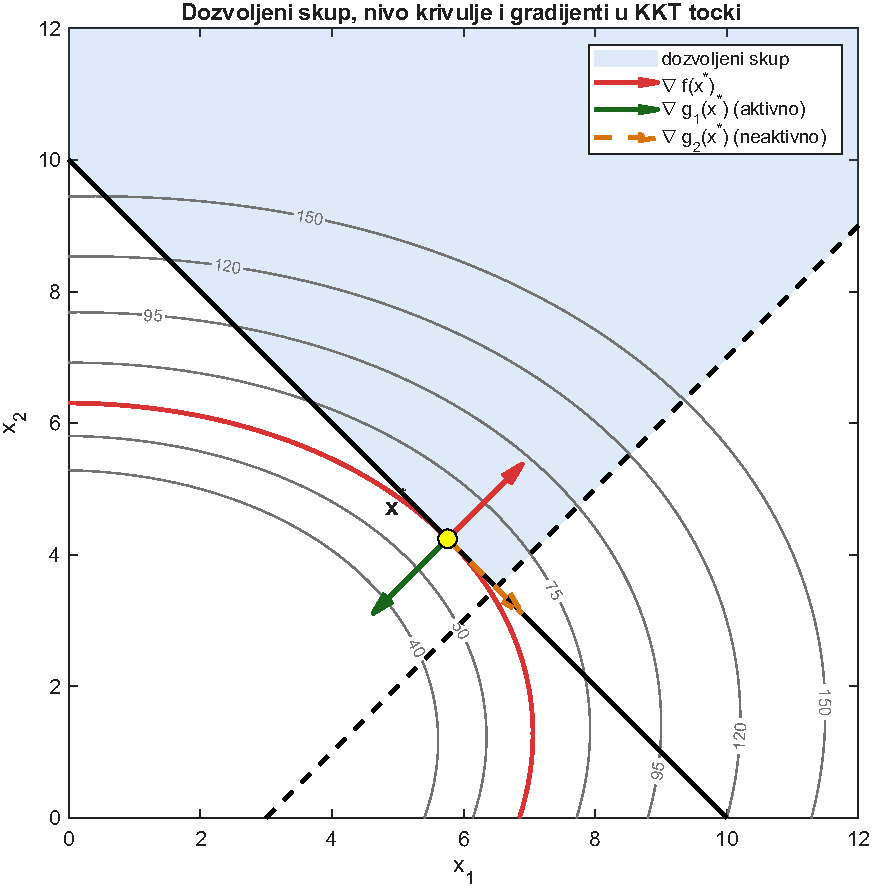
\includegraphics[width=0.78\textwidth]{figures/zad1_kkt.pdf}
  \caption{Dozvoljeni skup (plavo), nivo krivulje funkcije cilja, aktivno
  ograničenje (puna crta), neaktivno ograničenje (crtkano) te gradijenti
  funkcije cilja i obaju ograničenja u točki $x^\star$. Crvena krivulja je nivo
  krivulja $f(x) = p^\star$.}
  \label{fig:z1}
\end{figure}

\subsection{Numeričko rješenje u MATLAB-u}
\label{sec:zad1:matlab}

Problem je riješen dvama neovisnim putevima, funkcijom \texttt{quadprog} iz
Optimization Toolboxa i modeliranjem u YALMIP-u. Oba vraćaju
\begin{equation}
  x^\star = (5{,}757576,\; 4{,}242424)^{\mathsf T}, \qquad
  \lambda^\star = (12{,}242424,\; 0)^{\mathsf T},
\end{equation}
uz odstupanje od analitičkog rješenja \eqref{eq:z1sol} reda $10^{-11}$
(\texttt{quadprog}) odnosno $10^{-16}$ (YALMIP). Lagrangeovi množitelji koje
vraćaju solveri poklapaju se s onima izračunatima iz KKT sustava, što je i
očekivano: za konveksan QP množitelji su jedinstveni kad su gradijenti aktivnih
ograničenja linearno nezavisni, a ovdje je aktivno samo jedno ograničenje.

\subsection{Lagrangeov dualni problem}
\label{sec:zad1:dual}

Dualna funkcija je $g(\lambda) = \min_x L(x,\lambda)$. Kako je $H \succ 0$,
minimizacija po $x$ ima zatvorenu formu: iz $\nabla_x L = Hx + c + A^{\mathsf T}\lambda = 0$
slijedi $x = -H^{-1}(c + A^{\mathsf T}\lambda)$, pa je
\begin{equation}
  g(\lambda) = -\tfrac{1}{2}\,(c + A^{\mathsf T}\lambda)^{\mathsf T} H^{-1} (c + A^{\mathsf T}\lambda) - \lambda^{\mathsf T}b .
  \label{eq:dualfun}
\end{equation}
Dualni problem je $\max_{\lambda \ge 0} g(\lambda)$; to je konkavna maksimizacija,
dakle konveksan problem \cite[str.~24]{jokic_dualnost}.

Numeričko rješavanje \eqref{eq:dualfun} daje
\begin{equation}
  \lambda^\star = (12{,}242424,\; 0)^{\mathsf T}, \qquad d^\star = 60{,}606061 ,
\end{equation}
što se poklapa s množiteljima iz (b) i (d). Dualni jaz je
$p^\star - d^\star \approx 10^{-8}$, dakle numerički nula. Jaka dualnost je i
očekivana: problem je konveksan, a ograničenja su afina, pa je Slaterov uvjet
zadovoljen već postojanjem strogo dopustive točke \cite[str.~28]{jokic_dualnost}.

\subsection{Osjetljivost optimalne vrijednosti na perturbacije ograničenja}
\label{sec:zad1:osjetljivost}

Lagrangeovi množitelji imaju izravnu interpretaciju kao osjetljivost optimalne
vrijednosti na popuštanje ograničenja:
\begin{equation}
  \frac{\partial p^\star}{\partial b_i} = -\lambda_i^\star .
  \label{eq:sens}
\end{equation}
Uvrštavanjem rezultata \eqref{eq:z1sol}:
\begin{equation}
  \frac{\partial p^\star}{\partial b_1} = -12{,}242424, \qquad
  \frac{\partial p^\star}{\partial b_2} = 0 .
\end{equation}

Numerička provjera centralnom razlikom uz $\varepsilon = 10^{-6}$ daje
$-12{,}242424$ i $0{,}000000$, u skladu s \eqref{eq:sens}.

Tumačenje je sljedeće. Povećanje $b_1$ za $\Delta$ znači popuštanje aktivnog
ograničenja, pa optimalna vrijednost pada za približno $12{,}24\,\Delta$ --- to je
ograničenje koje stvarno „košta“. Ograničenje \eqref{eq:z1g2} je neaktivno, pa
njegova mala perturbacija ne mijenja rješenje: postoji rezerva od
$1{,}484848$ prije nego što ono postane aktivno, i tek za perturbacije veće od te
rezerve odnos \eqref{eq:sens} prestaje vrijediti. Relacija je lokalna i vrijedi
dok se skup aktivnih ograničenja ne promijeni.


% 02 — Zadatak 2: robustan QP uz nesigurne koeficijente (+-15 %).
% Struktura poglavlja; sadržaj popunjava writer uz citate iz rag query.

\section{Zadatak 2 --- robusno kvadratično programiranje}
\label{sec:zad2}

\subsection{Model nesigurnosti koeficijenata}
\label{sec:zad2:nesigurnost}

\subsection{Robusna formulacija problema}
\label{sec:zad2:formulacija}

\subsection{Rješenje robusnog problema}
\label{sec:zad2:rjesenje}

\subsection{Dozvoljeni skupovi za slučajne realizacije koeficijenata}
\label{sec:zad2:skupovi}

\subsection{Usporedba s nominalnim rješenjem}
\label{sec:zad2:usporedba}


% 03 — Zadatak 3: formulacija opt. problema, optimalna aproksimacija s ograničenjima.

\section{Zadatak 3 --- optimalna aproksimacija s ograničenjima}
\label{sec:zad3}

\subsection{Opis problema izgradnje ceste na neravnom terenu}
\label{sec:zad3:opis}

Cestu treba izgraditi na neravnom terenu poznate visine $h(x)$, $x \in [0, L]$.
Trošak izrade proporcionalan je količini materijala koju treba otkopati ili
dodati da bi se dobio profil ceste $y(x)$, uz ograničenja na nagib, na brzinu
promjene nagiba te uz zadane rubne uvjete \cite[str.~1]{jokic_zadatak}. Zadano je
\begin{equation}
  L = 10, \qquad h(x) = 0{,}0053x^4 - 0{,}095x^3 + 0{,}48x^2 - 0{,}3x + 1,
\end{equation}
uz $a = h(0) = 1$ i $b = h(L) = 4$, te dva slučaja:
slučaj A s $b_1 = 0{,}5$, $b_2 = 0{,}5$ i slučaj B s $b_1 = 0{,}5$, $b_2 = 0{,}2$.

\subsection{Diskretizacija i aproksimacija derivacija}
\label{sec:zad3:diskretizacija}

Interval $[0,L]$ dijeli se na $N$ podintervala duljine $\Delta x = L/N$, s
čvorovima $x_i = i\,\Delta x$, $i = 0,\dots,N$, pri čemu je $x_0 = 0$ i $x_N = L$.
Nepoznanice su visine ceste u čvorovima, $y_i = y(x_i)$.

Nagib se aproksimira prvom podijeljenom razlikom, a brzina promjene nagiba
ponovnom primjenom iste operacije:
\begin{equation}
  \nabla y_i = \frac{y_i - y_{i-1}}{\Delta x},\quad i = 1,\dots,N, \qquad
  \nabla^2 y_i = \frac{\nabla y_i - \nabla y_{i-1}}{\Delta x}
               = \frac{y_i - 2y_{i-1} + y_{i-2}}{\Delta x^2},\quad i = 2,\dots,N .
  \label{eq:z3diff}
\end{equation}
Obje su aproksimacije \emph{linearne} u nepoznanicama $y_i$, što je ključno za
klasifikaciju problema.

\subsection{Formulacija optimizacijskog problema}
\label{sec:zad3:formulacija}

Količina premještenog materijala na $i$-tom podintervalu proporcionalna je
apsolutnoj razlici visina, jer se i otkopavanje i nasipavanje jednako plaćaju.
Ukupni trošak je stoga
\begin{equation}
  J(y) = \sum_{i=0}^{N} \lvert y_i - h(x_i)\rvert \,\Delta x,
  \label{eq:z3cost}
\end{equation}
što je diskretizacija integrala $\int_0^L |y(x)-h(x)|\,\mathrm{d}x$, dakle
$\ell_1$ norma odstupanja. Problem glasi
\begin{align}
  \min_{y \in \mathbb{R}^{N+1}}\quad & \sum_{i=0}^{N} \lvert y_i - h_i\rvert\,\Delta x \label{eq:z3a}\\
  \text{uz}\quad & \lvert y_i - y_{i-1}\rvert \le b_1 \Delta x, && i = 1,\dots,N, \label{eq:z3b}\\
                 & \lvert y_i - 2y_{i-1} + y_{i-2}\rvert \le b_2 \Delta x^2, && i = 2,\dots,N, \label{eq:z3c}\\
                 & y_0 = a, \quad y_N = b . \label{eq:z3d}
\end{align}

\subsection{Klasifikacija problema}
\label{sec:zad3:klasa}

Funkcija cilja \eqref{eq:z3a} je konveksna ali nije glatka, dok su sva
ograničenja linearna. Standardnom \emph{epigrafskom reformulacijom} uvode se
pomoćne varijable $t_i$ uz
\begin{equation}
  y_i - h_i \le t_i, \qquad -(y_i - h_i) \le t_i,
\end{equation}
što je ekvivalentno $t_i \ge |y_i - h_i|$, a cilj postaje $\sum_i t_i \Delta x$.
Time i cilj i sva ograničenja postaju linearni, pa je riječ o
\textbf{linearnom programu} (LP) \cite[str.~30]{jokic_lpqp} s $2(N+1)$ varijabli.
Apsolutne vrijednosti u \eqref{eq:z3b}--\eqref{eq:z3c} razlažu se na po dvije
linearne nejednakosti na isti način.

Da je trošak bio proporcionalan \emph{kvadratu} odstupanja, problem bi bio QP;
$\ell_1$ mjera je ovdje fizikalno ispravna jer je količina zemlje razmjerna
apsolutnoj, a ne kvadriranoj razlici. Ta razlika ima i praktičnu posljedicu:
$\ell_1$ cilj daje rješenja koja se na dijelovima \emph{točno} poklapaju s
terenom, dok bi $\ell_2$ cilj odstupanje razmazao po cijeloj domeni.

\subsection{Rezultati}
\label{sec:zad3:rezultati}

Problem je riješen funkcijom \texttt{linprog} za sva četiri tražena slučaja.
Svi su riješeni do optimalnosti; rezultati su u tablici~\ref{tab:z3}, a profili
na slici~\ref{fig:z3}.

\begin{table}[htbp]
  \centering
  \caption{Rezultati za četiri slučaja. Aktivna ograničenja pokazuju koje
  ograničenje oblikuje rješenje.}
  \label{tab:z3}
  \begin{tabular}{llccccc}
    \hline
    Slučaj & $N$ & $b_1$ & $b_2$ & trošak & aktivnih nagiba & aktivnih zakrivljenosti \\
    \hline
    A & $20$  & $0{,}5$ & $0{,}5$ & $1{,}916180$ & $10/20$  & $3/19$  \\
    A & $100$ & $0{,}5$ & $0{,}5$ & $1{,}965940$ & $51/100$ & $35/99$ \\
    B & $20$  & $0{,}5$ & $0{,}2$ & $2{,}453727$ & $5/20$   & $12/19$ \\
    B & $100$ & $0{,}5$ & $0{,}2$ & $2{,}506047$ & $25/100$ & $73/99$ \\
    \hline
  \end{tabular}
\end{table}

\begin{figure}[htbp]
  \centering
  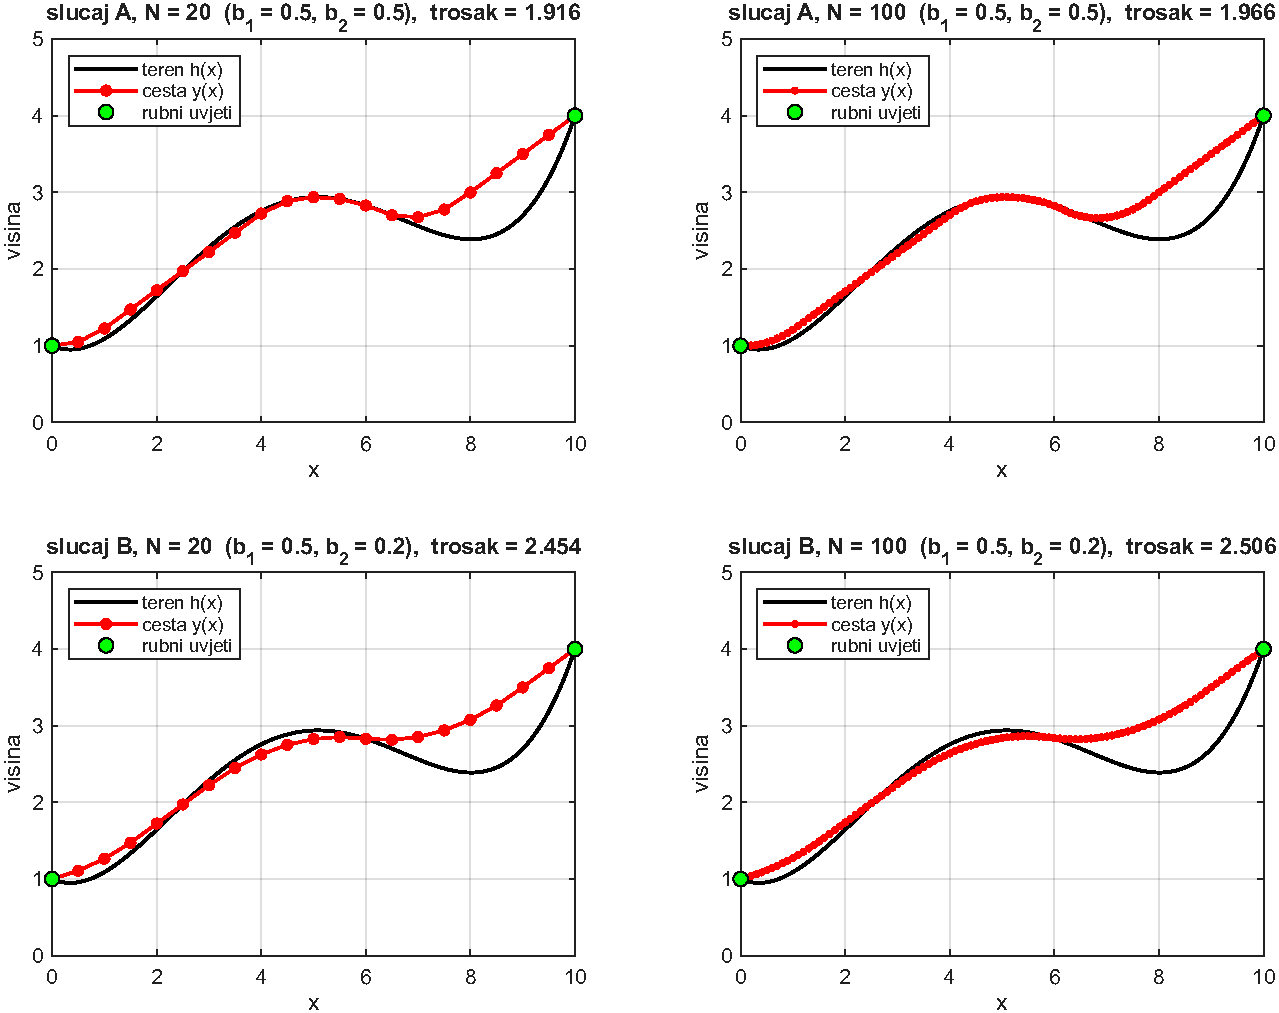
\includegraphics[width=\textwidth]{figures/zad3_cesta.pdf}
  \caption{Teren $h(x)$ (crno) i optimalni profil ceste $y(x)$ (crveno) za sva
  četiri slučaja. Zelene točke su rubni uvjeti.}
  \label{fig:z3}
\end{figure}

U svim slučajevima rubni uvjeti su zadovoljeni do strojne točnosti, a
ograničenja \eqref{eq:z3b}--\eqref{eq:z3c} dosegnuta su točno na svojim
granicama ($\max|\nabla y| = 0{,}5$, $\max|\nabla^2 y| = b_2$), što potvrđuje da
su ona doista aktivna i da rješenje leži na rubu dozvoljenog skupa.

\subsection{Usporedba slučajeva i utjecaj diskretizacije}
\label{sec:zad3:diskusija}

\paragraph{Utjecaj ograničenja $b_2$.} Slučaj B je stroži i skuplji: trošak raste
s $1{,}92$ na $2{,}45$ pri $N=20$, dakle za oko $28\,\%$. Struktura rješenja se
kvalitativno mijenja --- u slučaju A dominira ograničenje nagiba (aktivno na
polovici čvorova), dok u slučaju B prevladava ograničenje zakrivljenosti
($73/99$ aktivnih pri $N=100$). Profil u slučaju B je vidljivo glađi jer se
nagib ne smije mijenjati brzo, pa cesta ne može tako vjerno pratiti teren.

\paragraph{Utjecaj diskretizacije.} Prijelaz s $N=20$ na $N=100$ mijenja trošak
tek u trećoj znamenki ($1{,}916 \to 1{,}966$ i $2{,}454 \to 2{,}506$, oko
$2\,\%$). Rješenje dakle konvergira i grubljom mrežom već je dobro
aproksimirano. Blagi porast je očekivan: finija mreža bolje aproksimira integral
i uz to nameće ograničenja u više točaka, pa je dozvoljeni skup nešto uži.

\paragraph{Oblik rješenja.} Na dijelovima gdje teren zadovoljava ograničenja
cesta ga prati gotovo točno, čime je trošak lokalno nula. Odstupanje se
koncentrira ondje gdje teren mijenja smjer prebrzo --- osobito u udolini oko
$x \approx 8$, gdje teren pada, a cesta mora nastaviti rasti kako bi dosegla
rubni uvjet $y(L) = 4$ uz ograničen nagib. Upravo taj dio nosi najveći dio
troška i u oba slučaja određuje rješenje.


% 04 — Zadatak 4: robusna stabilizacija prekidačkog (switching) sustava.

\section{Zadatak 4 --- robusna stabilizacija prekidačkog sustava}
\label{sec:zad4}

\subsection{Opis vremenski promjenjivog sustava}
\label{sec:zad4:opis}

Promatra se vremenski promjenjiv sustav \cite[str.~2]{jokic_zadatak}
\begin{equation}
  \dot{x}(t) = A(t)\,x(t) + B\,u(t), \qquad
  A(t) = \begin{cases}
    A_{\text{parno}}, & \lfloor t \rfloor \text{ paran},\\
    A_{\text{neparno}}, & \lfloor t \rfloor \text{ neparan},
  \end{cases}
  \label{eq:z4sys}
\end{equation}
uz
\begin{equation}
  A_{\text{parno}} = \begin{bmatrix} -1 & -\tfrac{1}{6}\pi \\[2pt] \tfrac{3}{2}\pi & -1 \end{bmatrix}, \qquad
  A_{\text{neparno}} = \begin{bmatrix} -1 & -\tfrac{3}{2}\pi \\[2pt] \tfrac{1}{6}\pi & -1 \end{bmatrix}.
\end{equation}
Riječ je o hibridnom sustavu sa skokovitom promjenom dinamike u cjelobrojnim
trenucima; između dva prekapčanja sustav je linearan i vremenski invarijantan.

\subsection{Stabilnost pojedinih dinamičkih modova}
\label{sec:zad4:modovi}

Za matricu oblika $\left[\begin{smallmatrix} -1 & -\alpha \\ \beta & -1 \end{smallmatrix}\right]$
karakteristični polinom je $(\lambda+1)^2 + \alpha\beta = 0$, pa je
$\lambda = -1 \pm \mathrm{i}\sqrt{\alpha\beta}$. U oba moda umnožak
izvandijagonalnih elemenata je jednak,
\begin{equation}
  \alpha\beta = \frac{\pi}{6}\cdot\frac{3\pi}{2} = \frac{\pi^2}{4},
\end{equation}
pa oba moda imaju iste svojstvene vrijednosti
\begin{equation}
  \lambda_{1,2} = -1 \pm \mathrm{i}\,\frac{\pi}{2} .
\end{equation}
Realni dio je $-1 < 0$, dakle \textbf{obje su matrice Hurwitzove} i oba su
dinamička moda asimptotski stabilna \cite[str.~5]{jokic_ljapunov}.

\subsection{Simulacija sustava u otvorenom krugu}
\label{sec:zad4:simulacija}

Stabilnost pojedinih modova \emph{ne} povlači stabilnost prekidačkog sustava.
Kako je prekapčanje periodično s periodom $2$ (jedna sekunda u svakom modu),
stabilnost se ispituje monodromijskom matricom preko jednog perioda:
\begin{equation}
  \Phi = e^{A_{\text{neparno}}\cdot 1}\,e^{A_{\text{parno}}\cdot 1} .
\end{equation}
Sustav je stabilan ako i samo ako je spektralni radijus $\rho(\Phi) < 1$.
Izračun daje
\begin{equation}
  \operatorname{eig}(\Phi) = \{-1{,}218018,\; -0{,}015037\}, \qquad
  \rho(\Phi) = 1{,}218018 > 1 ,
\end{equation}
pa je prekidački sustav \textbf{nestabilan}. Floquetov eksponent je
$\tfrac{1}{2}\ln\rho = +0{,}098612$, dakle amplituda raste kao $e^{0{,}0986\,t}$.

Gornji lijevi i desni dio slike~\ref{fig:z4} potvrđuju zaključak: uz
$x(0) = (1,0)^{\mathsf T}$ stanja osciliraju s rastućom amplitudom, a trajektorija
se u prostoru stanja spiralno udaljava od ishodišta.

Objašnjenje je geometrijsko. Svaki mod sam za sebe rotira trajektoriju prema
ishodištu, ali dva moda rotiraju u različitim "smjerovima rastezanja". Prekapčanje
je vremenski usklađeno tako da svaki mod preuzme stanje u trenutku kad ga može
pojačati; energija koju jedan mod ukloni, drugi doda s viškom. Zato provjera
svojstvenih vrijednosti pojedinih modova nije dovoljna za prekidačke sustave.

\subsection{Sinteza statičkog regulatora}
\label{sec:zad4:regulator}

Uz $B = (1,0)^{\mathsf T}$ traži se statički regulator $u = Kx$ takav da je
zatvoreni krug $\dot{x} = (A(t) + BK)x$ eksponencijalno stabilan.

Dovoljan uvjet je postojanje \emph{zajedničke} kvadratne Ljapunovljeve funkcije
$V(x) = x^{\mathsf T}Px$, $P \succ 0$, za koju $\dot V < 0$ u oba moda
\cite[str.~4]{jokic_ljapunov}:
\begin{equation}
  (A_i + BK)^{\mathsf T}P + P(A_i + BK) \prec 0, \qquad i \in \{\text{parno}, \text{neparno}\} .
  \label{eq:z4lmi}
\end{equation}
Postoji li takav par $(P,K)$, zatvoreni krug je eksponencijalno stabilan za
\emph{proizvoljno} prekapčanje, ne samo za ovo periodično --- a to je jače od
onoga što zadatak traži.

Uvjet \eqref{eq:z4lmi} je bilinearan u $(P,K)$, no supstitucijom $Q = P^{-1}$ i
$Y = KQ$ prelazi u linearne matrične nejednakosti
\begin{equation}
  A_iQ + QA_i^{\mathsf T} + BY + Y^{\mathsf T}B^{\mathsf T} \prec 0, \quad Q \succ 0,
  \qquad K = YQ^{-1},
  \label{eq:z4lmi2}
\end{equation}
što je standardni put preko semidefinitnog programiranja \cite[str.~23]{jokic_qcpsdp}.
Na korištenom sustavu nije bio instaliran SDP rješavač, pa je certifikat izveden
analitički --- za sustav drugog reda to je izvedivo u zatvorenoj formi.

Uz $P = I$ i $K = [\,k_1\;\; k_2\,]$ zatvoreni krug ima oblik
$A_i + BK = \left[\begin{smallmatrix} -1+k_1 & c_i \\ \beta_i & -1 \end{smallmatrix}\right]$,
gdje je $c_{\text{parno}} = k_2 - \pi/6$, $\beta_{\text{parno}} = 3\pi/2$ te
$c_{\text{neparno}} = k_2 - 3\pi/2$, $\beta_{\text{neparno}} = \pi/6$. Tada je
\begin{equation}
  (A_i+BK)^{\mathsf T} + (A_i+BK) =
  \begin{bmatrix} 2(-1+k_1) & c_i + \beta_i \\ c_i + \beta_i & -2 \end{bmatrix} .
\end{equation}
Izbor
\begin{equation}
  k_2 = -\frac{4\pi}{3}
\end{equation}
poništava izvandijagonalni član parnog moda, pa on postaje dijagonalan i
negativno definitan čim je $k_1 < 1$. Za neparni mod uvjet negativne
definitnosti (pozitivna determinanta uz negativan trag) daje
\begin{equation}
  -4(-1+k_1) > \left(c_{\text{neparno}} + \beta_{\text{neparno}}\right)^2
  \quad\Longrightarrow\quad
  k_1 < 1 - \frac{16\pi^2}{9} = -16{,}545963 .
  \label{eq:z4bound}
\end{equation}

Odabrano je
\begin{equation}
  \boxed{\;K = \left[\,-20 \quad -\tfrac{4\pi}{3}\,\right] = [\,-20 \quad -4{,}188790\,].\;}
\end{equation}

Numerička provjera potvrđuje granicu \eqref{eq:z4bound}: za $k_1 = -16{,}6$ uvjet
je zadovoljen, a za $k_1 = -16{,}5$ nije. Uz odabrani $K$ i $P = I$ dobiva se

\begin{table}[htbp]
  \centering
  \caption{Certifikat stabilnosti zatvorenog kruga uz $P = I$.}
  \label{tab:z4}
  \begin{tabular}{lcc}
    \hline
    Mod & $\operatorname{eig}(A_i + BK)$ & $\operatorname{eig}\!\big((A_i+BK)^{\mathsf T}P + P(A_i+BK)\big)$ \\
    \hline
    parno    & $-19{,}820,\; -2{,}180$ & $-42{,}000,\; -2{,}000$ \\
    neparno  & $-20{,}764,\; -1{,}236$ & $-43{,}684,\; -0{,}316$ \\
    \hline
  \end{tabular}
\end{table}

Obje su matrice negativno definitne, čime je \eqref{eq:z4lmi} zadovoljen.
Iz $\dot V \le -0{,}3163\,V$ slijedi eksponencijalna ocjena
\begin{equation}
  \lVert x(t)\rVert \le \lVert x(0)\rVert\, e^{-0{,}1581\,t} .
\end{equation}

\subsection{Simulacija zatvorenog kruga}
\label{sec:zad4:zatvoreni}

Spektralni radijus monodromijske matrice zatvorenog kruga iznosi
$\rho(\Phi_{\text{cl}}) = 3{,}126\cdot10^{-2} \ll 1$, dakle amplituda se po
periodu smanji približno tridesetak puta. Donji dio slike~\ref{fig:z4} prikazuje
odziv uz isti početni uvjet $x(0) = (1,0)^{\mathsf T}$: stanja se ugase unutar
otprilike dvije sekunde, a trajektorija monotono ulazi u ishodište bez
oscilacija koje su obilježavale otvoreni krug.

\begin{figure}[htbp]
  \centering
  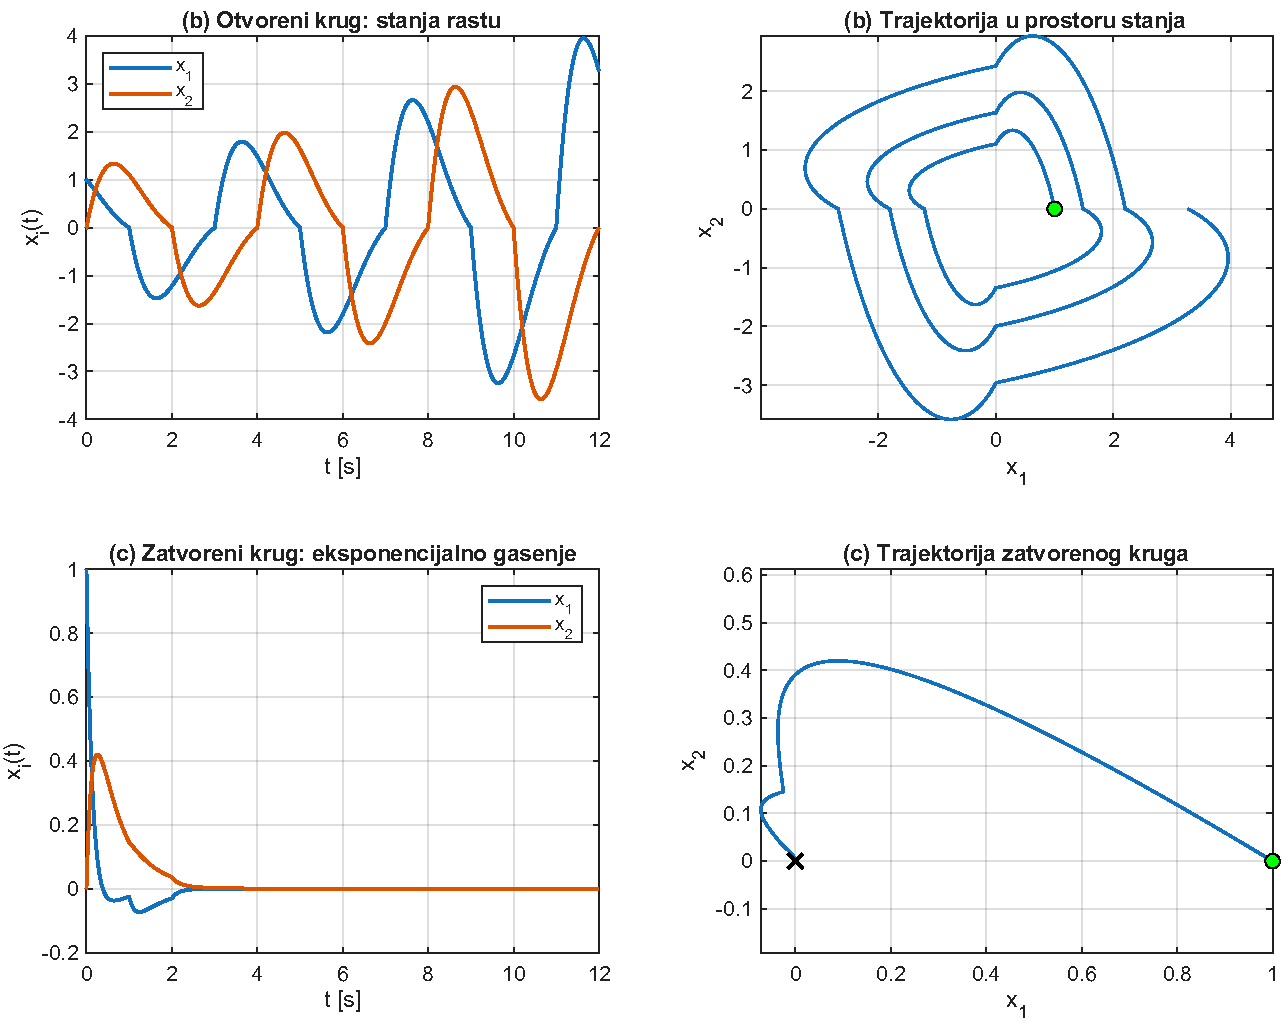
\includegraphics[width=\textwidth]{figures/zad4_switching.pdf}
  \caption{Prekidački sustav uz $x(0)=(1,0)^{\mathsf T}$. Gore: otvoreni krug ---
  stanja i trajektorija rastu unatoč tome što su oba moda Hurwitzova. Dolje:
  zatvoreni krug uz $u = Kx$ --- eksponencijalno gašenje.}
  \label{fig:z4}
\end{figure}

\subsection{Diskusija rezultata}
\label{sec:zad4:diskusija}

Zadatak dobro ilustrira tri stvari. Prvo, stabilnost svih pojedinačnih modova
nije dovoljna za stabilnost prekidačkog sustava --- ovdje su oba moda imala
identične svojstvene vrijednosti $-1 \pm \mathrm{i}\pi/2$, a sustav je ipak rastao
kao $e^{0{,}0986t}$. Drugo, ispravan alat je zajednička Ljapunovljeva funkcija:
ona daje certifikat neovisan o zakonu prekapčanja, dok analiza monodromijske
matrice vrijedi samo za točno ovaj periodični raspored. Treće, sinteza
regulatora prirodno se zapisuje kao LMI problem, čime ulazi u domenu
semidefinitnog programiranja i time u istu konveksnu okosnicu kao i prethodni
zadaci.

Cijena dobivenog rješenja je relativno velik pojačanje $k_1 = -20$. Uvjet
\eqref{eq:z4bound} pokazuje da je to nužno uz izbor $P = I$: granica
$1 - 16\pi^2/9 \approx -16{,}55$ posljedica je velikog raspona izvandijagonalnih
elemenata. Traženjem općenitijeg $P$ preko SDP-a mogao bi se dobiti manji
zahtjev na pojačanje, što je prirodan sljedeći korak ako bi upravljački signal
bio ograničen.


% zakljucak.

\section{Zaključak}
\label{sec:zakljucak}

U radu su riješena četiri zadatka koja pokrivaju raspon od uvjeta optimalnosti
za kvadratni program do sinteze regulatora za hibridni sustav.

U Zadatku~1 pokazano je da je zadani problem strogo konveksan kvadratni program,
pa su KKT uvjeti dovoljni za globalnu optimalnost. Analitičko rješenje
$x^\star = (190/33,\, 140/33)$ uz $\lambda^\star = (404/33,\, 0)$ potvrđeno je
trima neovisnim numeričkim putevima --- funkcijom \texttt{quadprog}, YALMIP-om i
rješavanjem dualnog problema --- uz dualni jaz reda $10^{-8}$. Osjetljivost
optimalne vrijednosti numerički se poklopila s $-\lambda^\star$, čime je
potvrđena interpretacija množitelja kao "cijene" ograničenja.

U Zadatku~2 pokazano je da intervalna nesigurnost koeficijenata ne mijenja klasu
problema: najgori slučaj po kvadru svodi se na član $r^{\mathsf T}|x|$, koji je
konveksan, pa robusna protuformulacija ostaje kvadratni program. Rezultat je
poučan --- nominalno rješenje, koje leži točno na granici, nedopustivo je u
$49{,}9\,\%$ slučajnih realizacija, dok robusno nije prekršilo ograničenja ni
jednom. Cijena te sigurnosti je porast funkcije cilja za oko $40\,\%$.

Zadatak~3 pokazao je koliko formulacija određuje ishod. Budući da je trošak
proporcionalan količini materijala, a ne njezinu kvadratu, prirodna mjera je
$\ell_1$ norma, što nakon epigrafske reformulacije daje linearni program.
Usporedba slučajeva pokazala je da strože ograničenje na promjenu nagiba
poskupljuje izvedbu za oko $28\,\%$ i mijenja strukturu rješenja: umjesto
ograničenja nagiba, rješenje počinje oblikovati ograničenje zakrivljenosti.
Prijelaz s $N = 20$ na $N = 100$ promijenio je trošak za tek oko $2\,\%$, pa je
gruba diskretizacija dovoljna za inženjersku procjenu.

Zadatak~4 dao je najizrazitiji rezultat: oba dinamička moda imaju identične
svojstvene vrijednosti $-1 \pm \mathrm{i}\pi/2$ i oba su Hurwitzova, a prekidački
sustav je ipak nestabilan, sa spektralnim radijusom monodromijske matrice
$1{,}218$. Time je pokazano da se stabilnost hibridnih sustava ne može ispitivati
mod po mod. Statički regulator $K = [-20,\; -4\pi/3]$ konstruiran je tako da uz
$P = I$ zadovoljava Ljapunovljevu nejednakost za oba moda, čime je zajamčena
eksponencijalna stabilnost \emph{za proizvoljno prekapčanje}, a ne samo za
zadani periodični raspored.

Zajednički zaključak jest da konveksnost nije tehnička sitnica nego glavni alat.
Ona je omogućila da se za Zadatak~1 tvrdi globalna optimalnost, da robusna
protuformulacija u Zadatku~2 ostane jednako lako rješiva kao nominalni problem,
da se Zadatak~3 svede na linearni program, i da se u Zadatku~4 problem sinteze
regulatora --- inače bilinearan --- supstitucijom $Q = P^{-1}$, $Y = KQ$ prevede
u konveksan skup linearnih matričnih nejednakosti.


\clearpage
% 05 — Prilog: MATLAB kod.

\section{Prilog --- MATLAB kod}
\label{sec:kod}

Sve numeričke vrijednosti i sve slike u ovom radu proizvedene su skriptama koje
slijede. Svaka je samostalna i pokreće se iz korijena projekta naredbom
\texttt{matlab -batch "run('src/zadatakN.m')"}. Skripte same razrješavaju
putanje relativno na vlastitu lokaciju, pa spremaju slike u \texttt{docs/figures/}
neovisno o tome iz kojeg se direktorija pozivaju.

Korištene su funkcije \texttt{quadprog} i \texttt{linprog} iz Optimization
Toolboxa, modeliranje u YALMIP-u te rješavač SeDuMi za semidefinitni program u
Zadatku~4.

\subsection{Zadatak 1 --- QP, KKT, dualnost, osjetljivost}
\label{sec:kod:z1}

\lstinputlisting[caption={\texttt{src/zadatak1.m}}, label={lst:z1}]{../src/zadatak1.m}

\clearpage
\subsection{Zadatak 2 --- robustan QP}
\label{sec:kod:z2}

\lstinputlisting[caption={\texttt{src/zadatak2.m}}, label={lst:z2}]{../src/zadatak2.m}

\clearpage
\subsection{Zadatak 3 --- optimalna aproksimacija s ograničenjima}
\label{sec:kod:z3}

\lstinputlisting[caption={\texttt{src/zadatak3.m}}, label={lst:z3}]{../src/zadatak3.m}

\clearpage
\subsection{Zadatak 4 --- robusna stabilizacija}
\label{sec:kod:z4}

\lstinputlisting[caption={\texttt{src/zadatak4.m}}, label={lst:z4}]{../src/zadatak4.m}


% ---- LITERATURA ----
\clearpage
\bibliographystyle{unsrt}
\bibliography{references}

\end{document}
